\documentclass[10pt,aspectratio=43,mathserif,table]{beamer} 
%设置为 Beamer 文档类型,设置字体为 10pt,长宽比为16:9,数学字体为 serif 风格
\batchmode
\usepackage{color}
\usepackage{graphicx}
\usepackage{animate}
\usepackage{hyperref}
\usepackage{subfigure}
%导入一些用到的宏包
\usepackage{amsmath,bm,amsfonts,amssymb,enumerate,epsfig,bbm,calc,color,ifthen,capt-of,multimedia,hyperref}
\usepackage{xeCJK} %导入中文包
\setCJKmainfont{SimHei} %字体采用黑体  Microsoft YaHei

\usetheme{Madrid} %主题
\usecolortheme{seahorse} %主题颜色

\usepackage[ruled,linesnumbered]{algorithm2e}
\usepackage{fancybox}
\usepackage{xcolor}
\usepackage{times}
\usepackage{listings}
\usepackage{algorithm} %format of the algorithm 

\usepackage{algorithmic} %format of the algorithm 

\usepackage{multirow} %multirow for format of table 

\usepackage{amsmath} 

\usepackage{xcolor}
\usepackage{booktabs}
\usepackage{colortbl}

\newcommand{\Console}{Console}
\lstset{ %
	backgroundcolor=\color{white},   % choose the background color
	basicstyle=\footnotesize\rmfamily,     % size of fonts used for the code
	columns=fullflexible,
	breaklines=true,                 % automatic line breaking only at whitespace
	captionpos=b,                    % sets the caption-position to bottom
	tabsize=4,
	commentstyle=\color{mygreen},    % comment style
	escapeinside={\%*}{*)},          % if you want to add LaTeX within your code
	keywordstyle=\color{blue},       % keyword style
	stringstyle=\color{mymauve}\ttfamily,     % string literal style
	numbers=left, 
	%	frame=single,
	rulesepcolor=\color{red!20!green!20!blue!20},
	% identifierstyle=\color{red},
	language=c
}

\setsansfont{Microsoft YaHei}
\setmainfont{Microsoft YaHei}
% \setbeamertemplate{navigation symbols}{}
% \usepackage{beamerthemeshadow}
\definecolor{mygreen}{rgb}{0,0.6,0}
\definecolor{mymauve}{rgb}{0.58,0,0.82}
\definecolor{mygray}{gray}{.9}
\definecolor{mypink}{rgb}{.99,.91,.95}
\definecolor{mycyan}{cmyk}{.3,0,0,0}

%题目,作者,学校,日期
\title{机器学习算法概述及其应用场景}
%subtitle{\fontsize{9pt}{14pt}\textbf{利用公共网关的SMS生态系统的安全性描述}}
\author{主讲人: 张聪聪}
\institute{\fontsize{8pt}{14pt}华润智慧能源有限公司}
\date{\today}

%学校Logo
\pgfdeclareimage[height=0.5cm]{sustech-logo}{crp-logo.pdf}
\logo{\pgfuseimage{sustech-logo}\hspace*{0.3cm}}

% \AtBeginSection[]
% {
% \begin{frame}<beamer>
% 	\frametitle{\textbf{目录}}
% 	\tableofcontents[currentsection]
% \end{frame}
% }
% \AtBeginSubsection[]
% {
%    \begin{frame}[shrink]
%       \tableofcontents[sectionstyle=show/shaded,subsectionstyle=show/shaded/hide]
%    \end{frame}
% }
\AtBeginSection[]
{
    \begin{frame}
        \tableofcontents[currentsection]%hideallsubsections]
    \end{frame}
}
%\At
\beamerdefaultoverlayspecification{<+->}
% -----------------------------------------------------------------------------
\begin{document}
% -----------------------------------------------------------------------------
\frame{\titlepage}
\section[目录]{}   %目录
\begin{frame}[allowframebreaks]
	\frametitle{目录}
	\tableofcontents
\end{frame}

\section{大数据与人工智能}
\begin{frame}
	\frametitle{大物移云智}
	\begin{figure}[]
		\centering
		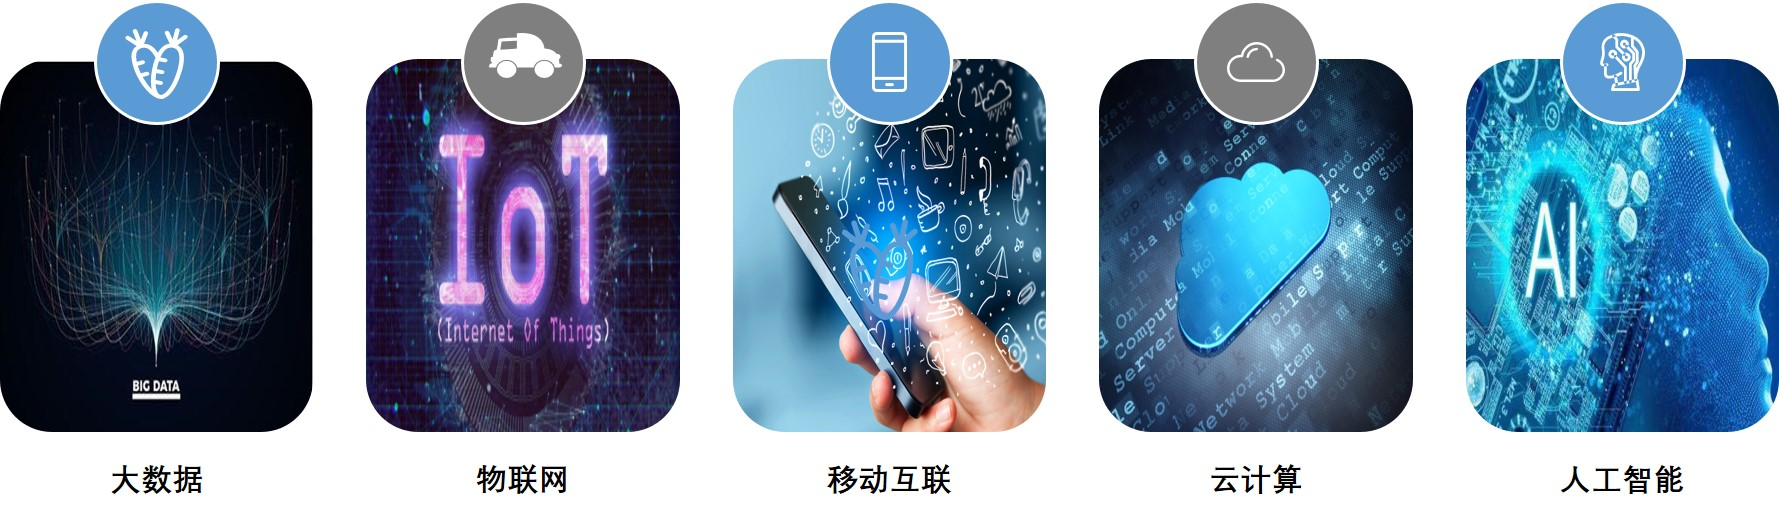
\includegraphics[width=1\textwidth]{figures/b_lot.jpg}
		%\caption{}
		\label{}
	\end{figure}
\end{frame}
\subsection{大数据}
%大数据定义
\begin{frame}
	\frametitle{大数据定义}
	\begin{block}{广义定义}
		\begin{itemize}
			\item<1-> 大数据是收集,组织,处理和收集大型数据集洞察所需的非传统策略和技术的总称。
			\item<1-> 大数据就是多,就是多。原来的设备存不下、算不动.
			\item<1-> 大数据,不是随机样本,而是所有数据;不是精确性,而是混杂性;不是因果关系,而是相关关系.
			\item<1-> 大数据,是指物理世界到数字世界的映射和提炼。通过发现其中的数据特征,从而做出提升效率的决策行为。
		\end{itemize}
	\end{block}
	\begin{block}<1->{狭义定义}
		大数据,是通过获取、存储、分析,从大容量数据中挖掘价值的一种全新的技术架构。
	\end{block}
	
\end{frame}
%大数据5v特点,为什么有大数据
\begin{frame}
	\frametitle{大数据特点}
	\begin{columns}[T] % align columns
		\begin{column}<0->{.48\textwidth}
			\begin{figure}[thpb]
				\centering
				\resizebox{1\linewidth}{!}{
					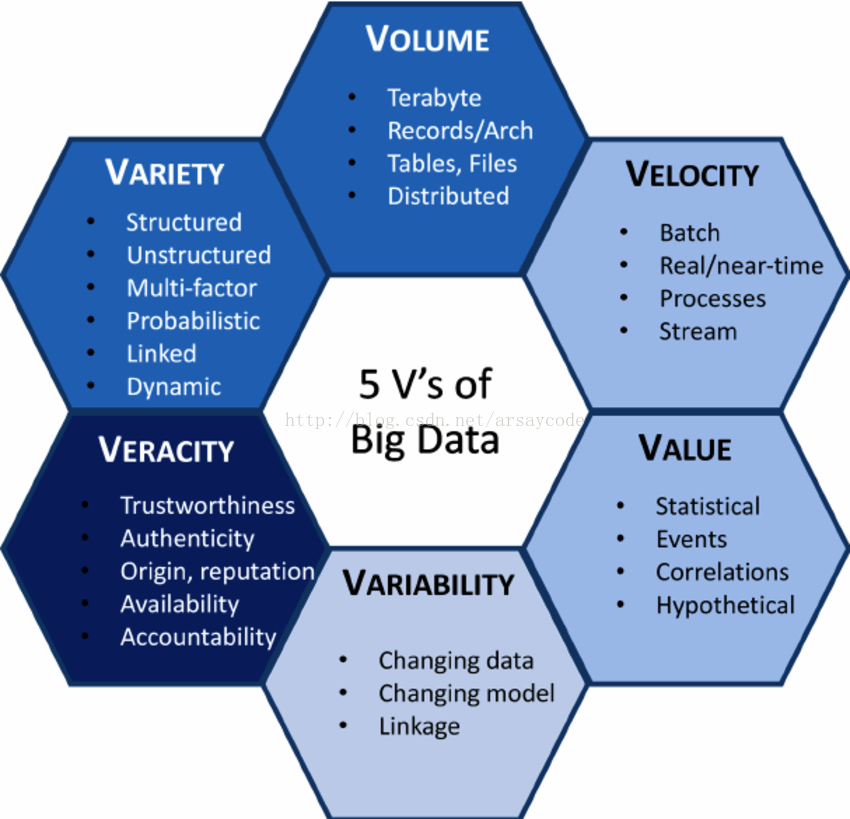
\includegraphics{figures/5v.png}
				}
				%\includegraphics[scale=1.0]{figurefile}
				%\caption{5v特点}
				\label{fig:campus}
			\end{figure}
		\end{column}%
		\hfill%
		\begin{column}<1->{.48\textwidth}
		\begin{block}<1->{5V}
			\begin{itemize}
				\item<1-> {\color{blue}\textbf{Volume}}:数据量大,包括采集、存储和计算的量都非常大。
				\item<1-> {\color{blue}\textbf{Variety}}:种类和来源多样化。包括结构化、半结构化和非结构化数据,具体表现为网络日志、音频、视频、图片、地理位置信息等等,多类型的数据对数据的处理能力提出了更高的要求。
				\item<1-> {\color{blue}\textbf{Value}}:数据价值密度相对较低,或者说是浪里淘沙却又弥足珍贵。
				\item<1-> {\color{blue}\textbf{Velocity}}:数据增长速度快,处理速度也快,时效性要求高。
				\item<1-> {\color{blue}\textbf{Velocity}}:数据的准确性和可信赖度,即数据的质量。
			\end{itemize}		
		\end{block}
		\end{column}%
	\end{columns}
\end{frame}
%大数据价值与应用场景
\begin{frame}
	\frametitle{大数据的价值与应用场景}
	\begin{columns}[c]
		\begin{column}<1->{.55\textwidth}
			\begin{figure}[thpb]
				\centering
				\resizebox{1\linewidth}{!}{
					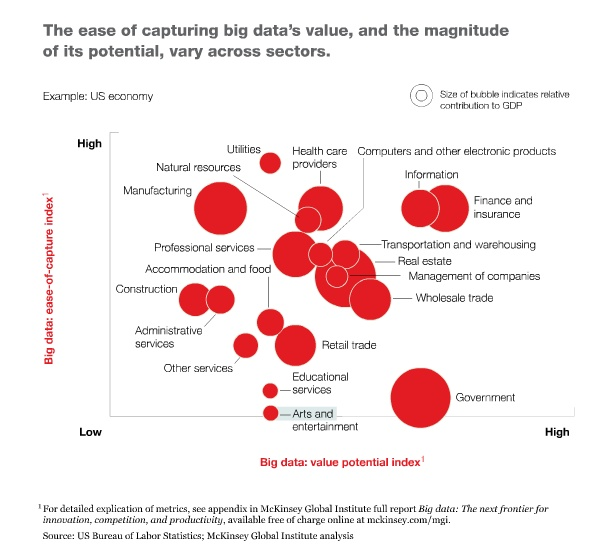
\includegraphics{figures/value.jpg}
				}
				%\includegraphics[scale=1.0]{figurefile}
				%\caption{5v特点}
				\label{fig:campus}
			\end{figure}
		\end{column}
		\hfill
		\begin{column}<1->{.40\textwidth}
		\begin{block}<1->{四类价值方法}
			\begin{itemize}
				\item<1-> 客户群体细分,然后为每个群体量定制特别的服务。
				\item<1-> 模拟现实环境,发掘新的需求同时提高投资的回报率。
				\item<1-> 加强部门联系,提高整条管理链条和产业链条的效率。
				\item<1-> 降低服务成本,发现隐藏线索进行产品和服务的创新。
			\end{itemize}
		\end{block}
		\end{column}
	\end{columns}
\end{frame}

\begin{frame}
	\frametitle{数据怎么来}
	\begin{columns}[c]
		\raggedright
		\begin{column}<1->{.55\textwidth}
			\begin{figure}[thpb]
				\centering
				\resizebox{1\linewidth}{!}{
					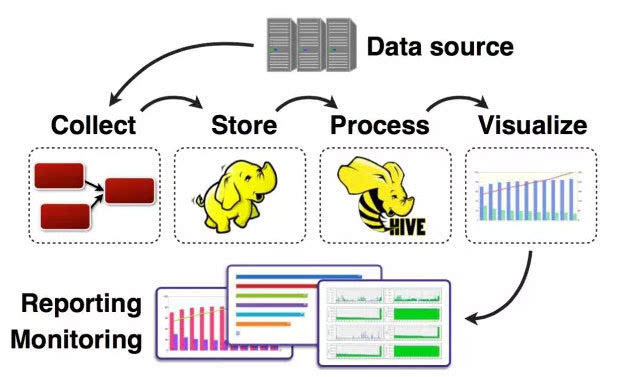
\includegraphics{figures/7step.jpg}
				}
				%\includegraphics[scale=1.0]{figurefile}
				%\caption{5v特点}
				\label{fig:campus}
			\end{figure}
		\end{column}
		\hfill
		\begin{column}<1->{.4\textwidth}
			\begin{block}<1->{大数据的六个环节}
			\begin{itemize}
				\item<1-> 数据提取
				\item<1-> 数据存储
				\item<1-> 数据清理
				\item<1-> 数据挖掘
				\item<1-> 数据分析
				\item<1-> 数据可视化
			\end{itemize}
		\end{block}
		\end{column}
	\end{columns}
	

\end{frame}
% \subsection{物联网}
% %物联网定义
% %物联网发展史
% %物联网特点
% %物联网应用
% \subsection{移动互联网}
% %移动互联网定义
% %移动互联网发展史
% %移动互联网特点
% %移动互联网应用
% \subsection{云计算}
% %云计算定义
% %云计算发展史
% %云计算特点
% %云计算应用
\subsection{人工智能}
\begin{frame}
	\begin{figure}[htbp]
		\centering
		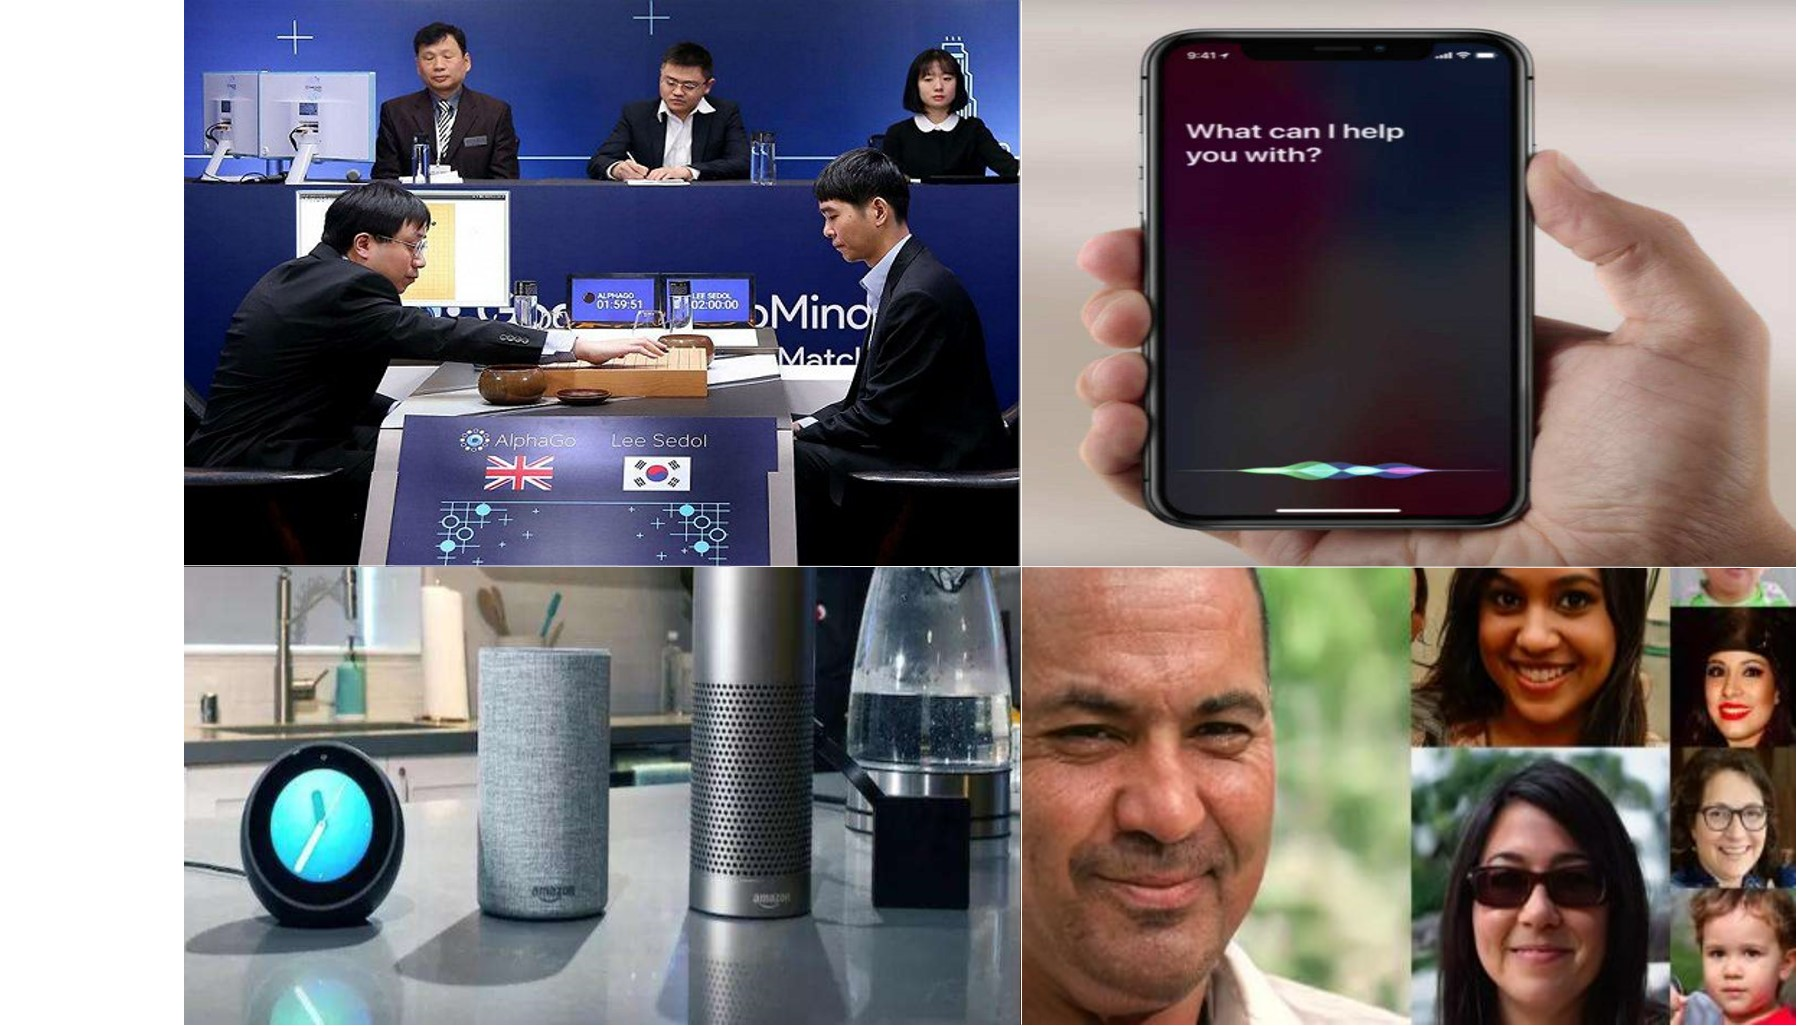
\includegraphics[width=0.9\textwidth]{figures/ai.jpg}
	\end{figure}
\end{frame}
%人工智能定义
\begin{frame}
	\frametitle{人工智能是什么}
	\begin{figure}[htbp]
		\centering
		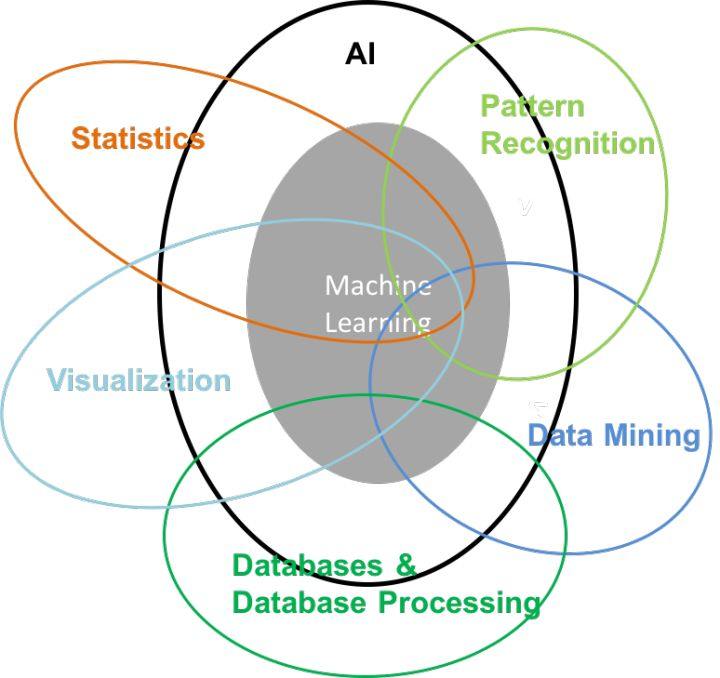
\includegraphics[width=0.3\textwidth]{figures/whatisai.jpg}
	\end{figure}
	\begin{block}{人工智能定义(Artificial Intelligence)}
		它是研究、开发用于模拟、延伸和扩展人的智能的理论、方法、技术及应用系统的一门新的技术科学
	\end{block}
\end{frame}
%人工智能的三个级别
\begin{frame}[allowframebreaks]
	\frametitle{人工智能的三个级别}

	\begin{figure}[htbp]
		\centering
		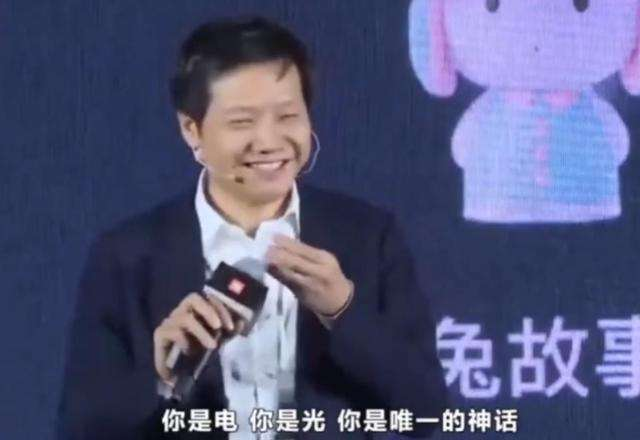
\includegraphics[scale=0.25]{figures/xiaomi.jpg}
	\end{figure}
	\begin{block}<1->{弱人工智能}
		也称限制领域人工智能(Narrow AI) 或应用型人工智能(Applied AI) , 指的是专注于且只能解决特定领域问题的人工智能。
	\end{block}
	\framebreak
	\begin{figure}[htbp]
		\centering
		
\includegraphics[scale=0.25]{figures/zhongjie.jpg}
	\end{figure}
	\begin{block}<1->{强人工智能}
		又称通用人工智能或完全人工智能, 指的是可以胜任人类所有工作的人工智能。
	\end{block}
	\framebreak
	\begin{figure}[htbp]
		\centering
		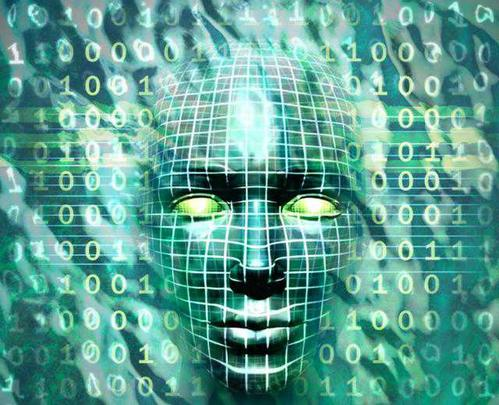
\includegraphics[scale=0.25]{figures/tianwang.jpg}
	\end{figure}
	\begin{block}<1->{超人工智能}
		假设计算机程序通过不断发展, 可以比世界上最聪明、 最有天赋的人类还聪明, 那么由此产生的人工智能系统就可以被称为超人工智能
	\end{block}
\end{frame}

%人工智能发展史
\begin{frame}[allowframebreaks]
	\frametitle{人工智能发展史}
	\begin{figure}[htbp]
		\centering
		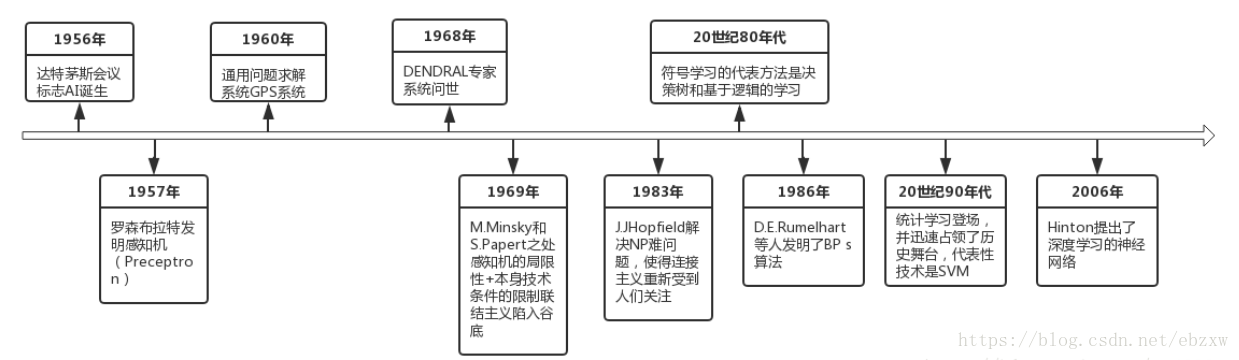
\includegraphics[width=0.8\textwidth]{figures/ailicheng.png}
	\end{figure}
	\begin{block}<1->{六个时期}
		\begin{itemize}
			\item<1->起步发展期:1956年—20世纪60年代初。
			\item<1-> 反思发展期:20世纪60年代—70年代初
			\item<1-> 应用发展期:20世纪70年代初—80年代中
			\item<1-> 低迷发展期:20世纪80年代中—90年代中
			\item<1-> 稳步发展期:20世纪90年代中—2010年
			\item<1-> 蓬勃发展期:2011年至今。
		\end{itemize}
	\end{block}
	\framebreak
	\begin{figure}
		\centering
		% Requires \usepackage{graphicx}
		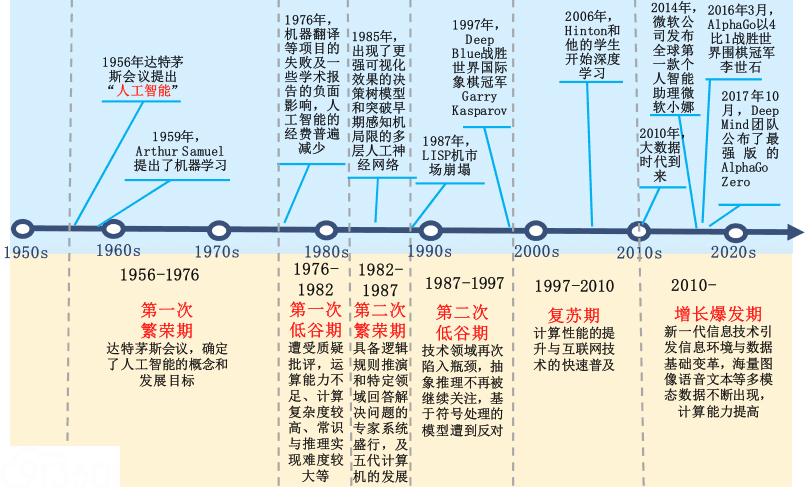
\includegraphics[width=0.9\paperwidth]{figures/licheng2.jpg}
		%\includegraphics[height=0.09\textwidth]{}
	  \end{figure}
\end{frame}

\begin{frame}[allowframebreaks]
	\frametitle{深度学习三巨头}
	% \begin{figure}
	% 	\centering
	% 	% Requires \usepackage{graphicx}
	% 	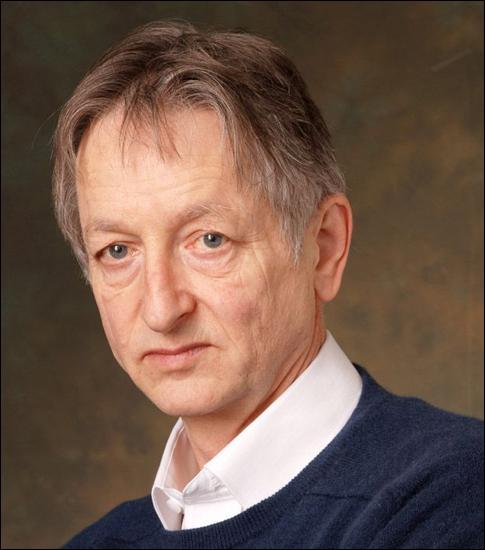
\includegraphics[width=0.3\paperwidth]{figures/hitton.jpeg}
	% 	%\includegraphics[height=0.09\textwidth]{}
	%   \end{figure}
	
	\begin{figure}
		\setlength{\abovecaptionskip}{0.cm}
		\setlength{\belowcaptionskip}{0.cm}
		\centering
		\subfigure[]{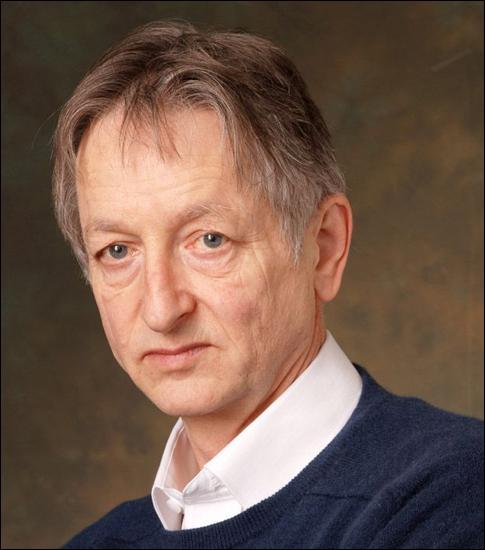
\includegraphics[width = 0.3\paperwidth]{figures/hitton.jpeg}}
		\subfigure[]{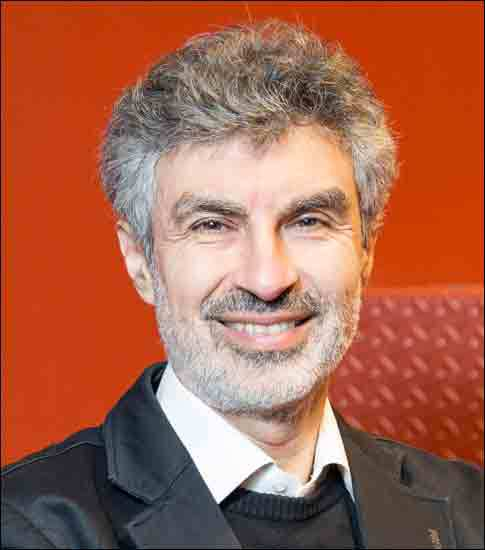
\includegraphics[width = 0.3\paperwidth]{figures/Yoshua_Bengio.jpeg}}
		\subfigure[]{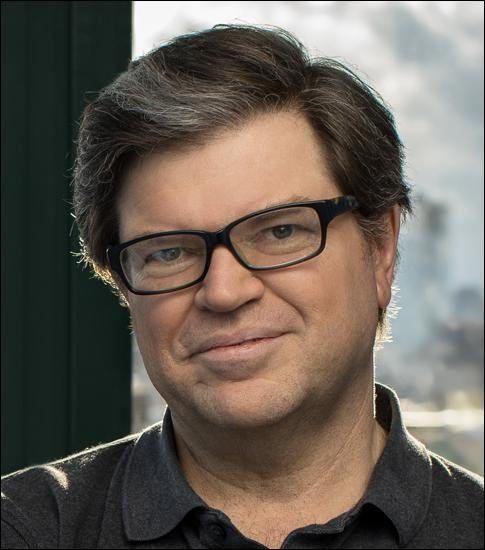
\includegraphics[width = 0.3\paperwidth]{figures/lecun.jpeg}}
		\caption{a)Geoffrey Hinton;b)Yoshua Bengio;c)Yann LeCun}
	\end{figure}
	\framebreak
	\begin{block}<1->{Geoffrey Hinton}
		\begin{enumerate}
			\item<1-> {\color{blue}\textbf{反向传播}}:证明了反向传播算法允许神经网络发现自己的数据内部表示,这使得使用神经网络成为可能网络解决以前被认为超出其范围的问题。
			\item<1-> {\color{blue}\textbf{玻尔兹曼机}}:这是第一个能够学习不属于输入或输出的神经元内部表示的神经网络之一。
			\item<1-> {\color{blue}\textbf{卷积神经网络的改进}}:2012 年,Hinton 和他的学生 Alex Krizhevsky 以及 Ilya Sutskever 通过 Rectified Linear Neurons 和 Dropout Regularization 改进了卷积神经网络,并在著名的 ImageNet 评测中将对象识别的错误率减半,在计算机视觉领域掀起一场革命。
		\end{enumerate}
	\end{block}
	\framebreak
	\begin{block}<1->{Yoshua Bengio}
		\begin{enumerate}
			\item<1-> {\color{blue}\textbf{序列概率模型}}:现代深度学习语音识别系统正在扩展这些概念。
			\item<1-> {\color{blue}\textbf{高维词嵌入和注意力模型}}:导致了机器翻译领域的突破,并构成了深度学习序列建模的关键组成部分;
			\item<1->  {\color{blue}\textbf{生成对抗网络}}:生成对抗网络(GANs),在计算机视觉和计算机图形学领域引发了一场革命。
		\end{enumerate}
	\end{block}
	\framebreak
	\begin{block}<1->{Yann LeCun}
		\begin{enumerate}
			\item<1-> {\color{blue}\textbf{卷积神经网络}}: 提出卷积神经网络(CNN),卷积神经网络已经成为计算机视觉、语音识别、语音合成、图像合成和自然语言处理领域的行业标准.
			\item<1->  {\color{blue}\textbf{改进反向传播算法}}:加速了反向传播算法;
			\item<1->  {\color{blue}\textbf{拓宽神经网络}}:他将神经网络发展为一种计算模型,用到一系列任务中,他早期工作中的一些概念已成为 AI 发展的基石。
		\end{enumerate}
	\end{block}
\end{frame}
%人工智能特点
%人工智能应用
\begin{frame}
	\frametitle{AI、机器学习、深度学习之间的关系}
	\begin{figure}[htbp]
		\centering
		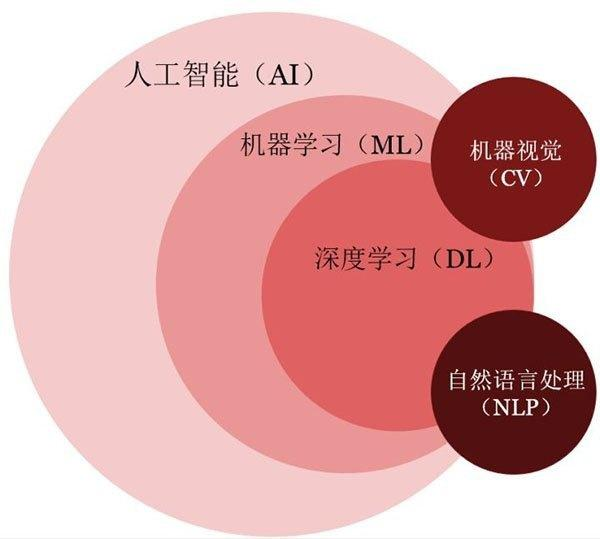
\includegraphics[width=0.5\paperwidth]{figures/guanxi.jpeg}
	\end{figure}
\end{frame}

\section{机器学习算法概述}
\subsection{算法}
%算法定义:三要素
\begin{frame}
	\frametitle{什么是算法}
	\begin{figure}[htbp]
		\centering
		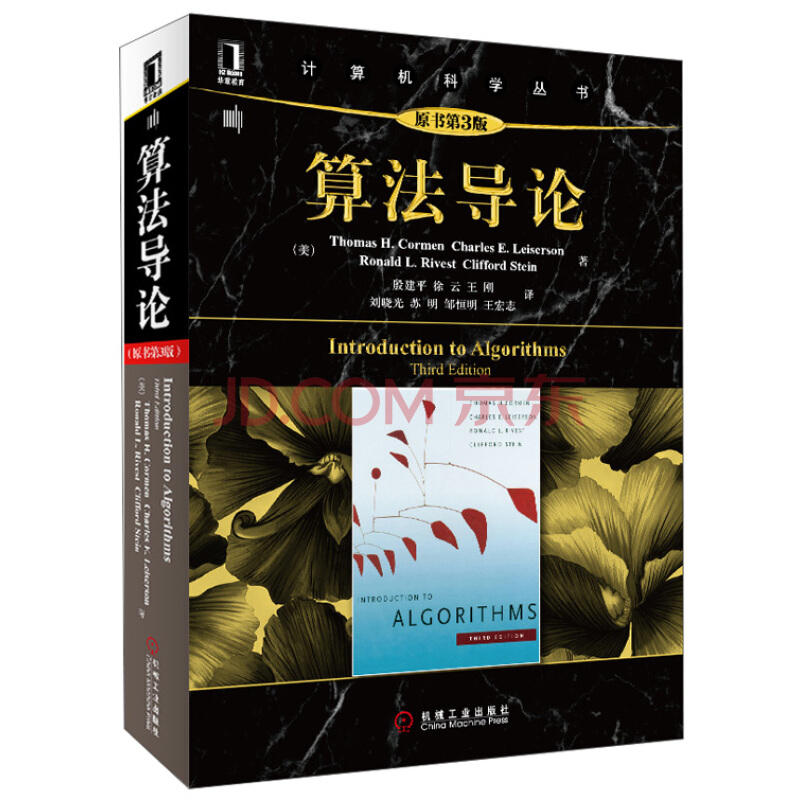
\includegraphics[width=0.3\paperwidth]{figures/algbook.jpg}
	\end{figure}

		\begin{block}<1->{算法}
				算法是任何良定义的{\color{blue}\textbf{计算过程}},该过程取某个值或值的集合作为{\color{blue}\textbf{输入}}并产生某个值或值的集合作为{\color{blue}\textbf{输出}}。
		\end{block}
\end{frame}
\begin{frame}
	\frametitle{算法伪代码}
    \begin{algorithm}[htb] 
		\caption{写算法名称} 
		\label{alg:Framwork} 
		\begin{algorithmic}[1] %这个1 表示从第一行开始显示行号,不写就不会显示行号
		\REQUIRE ~~\\ %算法的输入参数:Input
		输入1 \\
		输入2 \\
		\ENSURE ~~\\ %算法的输出:Output
		\STATE 输入1
		\STATE 输入2
		\RETURN 返回值; %算法的返回值
		\end{algorithmic}
		\end{algorithm}
\end{frame}
%时间复杂度空间复杂度
%算法表述形式:伪代码
%算法类别:来源于算法导论
\subsection{机器学习}
%机器学习是什么
%机器学习发展史
%机器学习学什么
%机器学习怎么学
%机器学习算法定义
%机器学习算法分类
%无监督学习:聚类
%监督学习
%强化学习
\section{机器学习算法应用场景}

\subsection{自然语言处理}

\subsection{语音识别}

\subsection{机器视觉}

\subsection{推荐系统}

% \section[目录]{}   %目录
% \begin{frame}{目录}
% \tableofcontents
% \end{frame}

% % -----------------------------------------------------------------------------
% \section{引言}  %引言
% \subsection{研究背景}
% \begin{frame}{研究背景}
% \begin{columns}[T] % align columns
% \begin{column}<0->{.40\textwidth}
% 	\begin{figure}[thpb]
% 		\centering
% 		\resizebox{1\linewidth}{!}{
% 			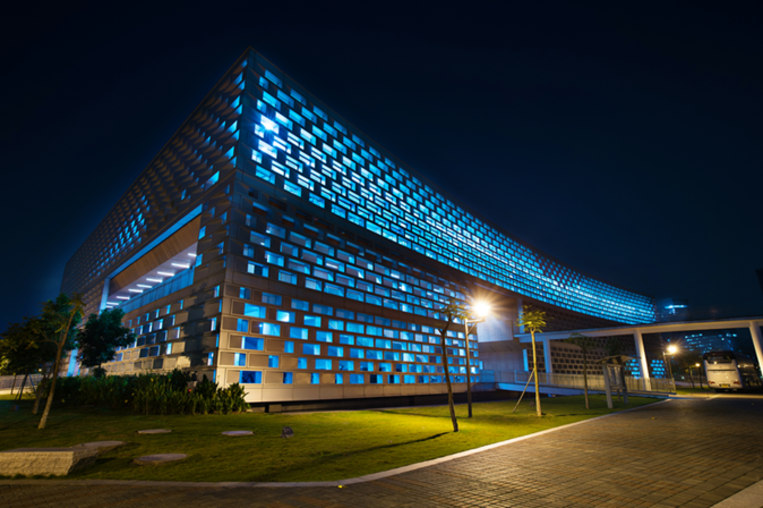
\includegraphics{figures/sustech.pdf}
% 		}
% 		%\includegraphics[scale=1.0]{figurefile}
% 		\caption{SUSTech Campus}
% 		\label{fig:campus}
% 	\end{figure}
% \end{column}%
% \hfill%
% \begin{column}<0->{.65\textwidth}
% 	\begin{itemize}
% 		\item<1-> 短信息(SMS)成为现代通讯的重要组成部分
% 		\begin{itemize}
% 			\item<1-> 很多组织或网站使用短信息作为身份验证的辅助通道
% 		\end{itemize}
% 		\item<1-> 现代短消息的发送,在抵达终端之前不接触蜂窝网络
% 		\begin{itemize}
% 			\item<1-> 短信息(SMS)成为现代通讯的重要组成部分
% 		\end{itemize}
% 	\end{itemize}
% \end{column}%
% \end{columns}
% \end{frame}
% \subsection{主要工作}
% \begin{frame}{主要工作}
% 完成这项工作需要如下步骤
% \begin{block}{具体步骤}
% \begin{itemize}
% 	\item<0->  对SMS数据进行迄今为止最大的挖掘分析
% 	\item<0->  评估良性短消息服务的安全态势
% 	\item<0->  刻画通过SMS网关进行的恶意行为
% \end{itemize}
% \end{block}
% \end{frame}

%  \begin{frame}
% \frametitle{OTT服务}
% \begin{figure}[!t]
% 	\centering
% 	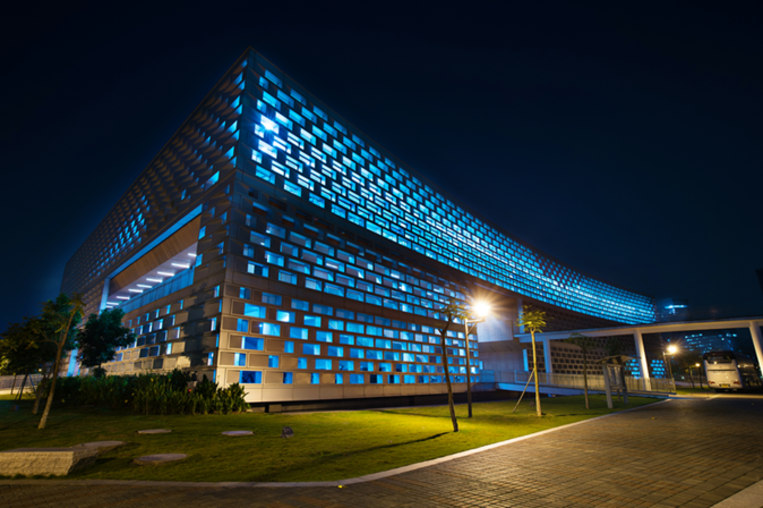
\includegraphics[width=2in]{figures/sustech.pdf}
% 	\caption{OTT服务}
% 	\label{figure3_OTT}
% \end{figure}
% \begin{center}
% 	OTT服务支持在数据网络上提供短信和语音等第三方服务。\\
% 	OTT可以使用云服务来存储和同步SMS到用户的其他设备。
% \end{center}

% \end{frame}



% \section{词表示模型}  %自我介绍

% \begin{frame}{词表示}
% 在NLP任务中,可以利用各种词表示模型,将“词”这种符号信息表示成数学上的向量形式。。将语义信息表示成稠密、低维的实值向量,这样就可以用计算向量之间相似度的方法(如余弦相似度),来计算语义的相似度。词的向量表示可以作为各种深度学习模型的输入来使用
% \begin{block}{词表示模型分类}
% 	直接表示模型
% 	\begin{itemize}
% 		\item<0-> One-Hot Representation
% 	\end{itemize}
	
% 	分布式表示模型
% 	\begin{itemize}
% 		\item<0-> 计数模型(基于共现矩阵)
% 		\item<0-> 预测模型(基于神经网络)
% 	\end{itemize}
% \end{block}
% \end{frame}


% \section{直接表示模型}
% \begin{frame}{One-Hot Representation}
% 最简单直接的词表示是One-Hot Representation。考虑一个词表$ \mathbb V $,里面的每一个词$ w_i $都有一个编号$ i\in \{1,...,n\} $,那么词$ w_i $的one-hot表示就是一个维度为n的向量,其中第$ i $个元素值非零,其余元素全为0。例如:
% \[  w_2=[0,1,0,...,0]^\top  \]
% \[  w_3=[0,0,1,...,0]^\top  \]
% \begin{block}{缺点}
% 	\begin{itemize}
% 		\item<0-> 彼此正交,不能反应词间的语义关系
% 		\item<0-> 稀疏表示,维度很高,和词典大小成正比
% 	\end{itemize}
% \end{block}
% \begin{center}
% 	\textcolor{mymauve}{仅仅是为了区分词,不包含语义信息,语义信息应该从上下文中挖掘}
% \end{center}
% \end{frame}


% \section{研究方法与数据集特征}
% \begin{frame}{研究方法与数据集特征}
% \begin{columns}[c] % align columns
% 	\begin{column}<0->{.5\textwidth}
% 		\vspace*{1cm}
% 		\begin{itemize}
% 			\item 使用Scrapy框架爬取公共网关
% 		\end{itemize}
	
% 		\begin{itemize}
% 			\item 收集8个公共短信网关在14个月的数据
% 		\end{itemize}
	
% 		\begin{itemize}
% 			\item 共抓取386,327条数据
% 		\end{itemize}
%     \end{column}%
% \hfill%	
% 	\begin{column}<0->{.40\textwidth}
% 		\begin{table}
% 			\caption{公共网关抓取的信息数}
% 			\footnotesize
% 			\rowcolors{1}{mygray}{white}
% 			\begin{tabular}{|c|c|}
% 				\hline
% 				\textbf{Site}           & \textbf{Messages}\\
% 				\hline
% 				receivesmsonline.net    &81313\\
% 				\hline
% 				receive-sms-online.info &69389\\
% 				\hline
% 				receive-sms-now.com     &63797\\
% 				\hline
% 				hs3x.com               &55499\\
% 				\hline
% 				receivesmsonline.com    &44640\\
% 				\hline
% 				receivefreesms.com      &37485\\
% 				\hline
% 				receive-sms-online.com  &27094\\
% 				\hline
% 				e-receivesms.com       &7107\\
% 				\hline
% 			\end{tabular}
% 		\end{table}
%     \end{column}%
% \end{columns}
% \end{frame}

% \begin{frame}
% \frametitle{消息聚类分析}
% \begin{block}{\textbf{基本思路}}
% 	\begin{itemize}
% 		\item<0-> 使用编辑距离矩阵将类似的消息归于一张连通图中。
% 		\item<0-> 使用固定值替换感兴趣的消息,如代码、email地址。
% 		\item<0-> 查找归一化距离小于阈值的消息,并确定聚类边界。
% 	\end{itemize}
% \end{block}

% \begin{block}{\textbf{实现步骤}}
% 	\begin{enumerate}
% 		\item<0-> 加载所有消息。
% 		\item<0-> 用固定的字符串替换数字、电子邮件和URL以预处理消息。
% 		\item<0-> 将预处理后的信息按字母排序。
% 		\item<0-> 通过使用编辑距离阈值(0.9)来确定聚类边界。
% 		\item<0-> 手动标记各个聚类,以确定服务提供者、消息类别等。
% 	\end{enumerate}
% \end{block}
% \end{frame}

% \section{算法和代码}
% \subsection{算法}
% \begin{frame}{算法}
% \begin{algorithm}[H]
% 	\caption{HOSVD}
% 	\small 
% 	\KwIn{HOSVD($\mathcal{X},R_{1},R_{2}.....R_{N}$) }
% 	\KwOut{ $\mathcal{G},A_{(1)},A_{(2)}......A_{(N)} $ }
	
% 	\For{$k=1$ to $N$ }
% 	{
% 		$A_{(n)}\leftarrow R_{n}$left singular matrix of $X_{(n)}$
% 	}
% 	$\mathcal{G}=\leftarrow \mathcal{X} \times A_{(1)}^{T} \times A_{(2)}^{T}...... \times A_{(N)}^{T}$\\
% 	\Return $\mathcal{G},A_{(1)},A_{(2)}......A_{(N)} $
% \end{algorithm}
% \end{frame}

% \subsection{代码}
% \begin{frame}[fragile]{代码}
% HOSVD在Python的代码实现和分析:
% \lstinputlisting[lastline=11,
% language=Python,
% frame=single,
% caption=First ten lines of some Python code,
% label=python]
% {HOSVD.py}
% \end{frame}


% \section{Future Work}
% \begin{frame}{Future Work}  %将来可做的方向
% \begin{itemize}
% \item<0-> Get more people to try this
% \item<0-> Benchmark the entire system in the wild
% \item<0-> Profit!
% \end{itemize}
% \end{frame}

% \begin{frame}{Thank you}
% \begin{center}
% \begin{minipage}{1\textwidth}
% 	\setbeamercolor{mybox}{fg=white, bg=black!50!blue}
%  \begin{beamercolorbox}[wd=0.70\textwidth, rounded=true, shadow=true]{mybox}
% \LARGE \centering Thank you for listening!  %结束语
% \end{beamercolorbox}
%  \end{minipage}
% \end{center}
% \end{frame}

% \begin{frame}{Q\&A}
% \begin{center}
% 	\begin{minipage}{1\textwidth}
% 		\setbeamercolor{mybox}{fg=white, bg=black!50!blue}
% 		\begin{beamercolorbox}[wd=0.70\textwidth, rounded=true, shadow=true]{mybox}
% 			\LARGE \centering  Questions?  %请求提问
% 		\end{beamercolorbox}
% 	\end{minipage}
% \end{center}
% \end{frame}

% -----------------------------------------------------------------------------
\end{document}
%文档结束